\include{settings}

\begin{document}	% начало документа

\include{titlepage}


% Содержание
\tableofcontents
\newpage



\section{Игровое приложение: "Побег из гробницы"}

Главный герой игры - археолог - оказывается в одном помещении с ожившей мумией, желающей расправиться с незваным гостем.\\



\subsection{Концепция игрового приложения "Побег из гробницы"}

Приложение являет собой логическую игру, в которой главному герою предстоит добраться до выхода из гробницы.\\

Приложение отрисовывает игровое поле, на которое помещаются два существа. Пользователь может управлять главным героем с помощью нажатия на клавиши-стрелки. Мумией управляет искусственный интеллект, заставляющий её двигаться по направлению к герою. Также на поле размещены преграды, мешающие существам пройти. Игра считается законченой, если пользователь довёл протагониста до выхода и не дал мумии догнать его.\\
Игровое поле составляется вне приложения в текстовом файле.\\

\subsection{Задание}

Разработать приложение под операционные системы Windows 7+ и Android, позволяющее играть в "Побег из гробницы". 

\subsection{Минимально работоспособный продукт}

Приложение, которое предоставляет возможность передвигать главного героя.

\subsection{Вывод}

Пояснён выбор темы курсового проекта. Описана концепция игры "Побег из гробницы". Определено задание.

%#######################################################################################################

\section{Проектирование графического приложения, реализующего игру "Побег из гробницы"}

\subsection{Проектирование библиотеки}

Приложение должно позволять игроку играть в "Побег из гробницы"\\

Библиотека - ядро приложения. Здесь содержатся основные классы, необ-
ходимые для представления игры. Для создания графического приложения
была выбрана библиотека LibGDX

\section{Реализация игры "Побег из гробницы"}

\subsection{Среда разработки}

Интегрированная среда разработки IntelliJ IDEA 2016.2.5.\\
Язык: Java 1.8.\\
Система автоматической сборки: Gradle 2.14.

\subsection{Реализация библиотеки}

Классы библиотеки объединены в пакет logic. Основные классы,
выделенные в библиотеке:\\

\begin{enumerate}
\item[1]  Класс Field. Содержит в себе игровое поле. Хранит массив из клеток, имеющих своё состояние.
\item[2]  Класс Cell. Клетка. Составляющая часть поля, доступно три состояния: свободная клетка, заблокированная клетка, выход из гробницы.
\item[3]  Класс Player. Хранит существ и хранит их координаты. Отвечает за их передвижение. 
\end{enumerate}


\subsection{Реализация графического приложения}

Для создания графического приложения была выбрана библиотека Swing.\\


На рисунке 1 представлен вариант игрового поля для игры "Побег из гробницы", где 0 - свободная клетка, 1 - преграда, 2 - выход:

\begin{figure}[H]
	\begin{center}
		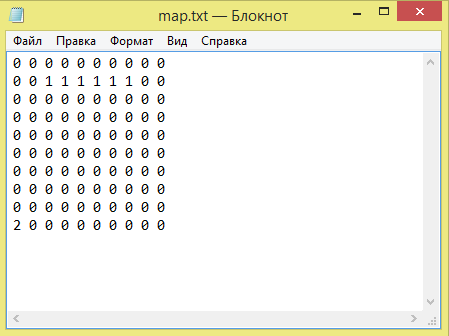
\includegraphics[scale=0.7]{image/map.png}
		\caption{Вручную созданное поле для игры.} 
		\label{pic:pic_name} % название для ссылок внутри кода
	\end{center}
\end{figure}

На рисунке 2 изображено соответствующая ему графическая интерпретация. Положение главного героя и мумии задано пользователем. На данный момент преграды и выход никак не обозначены, что будет исправлено в скорейшем времени. 

\begin{figure}[H]
	\begin{center}
		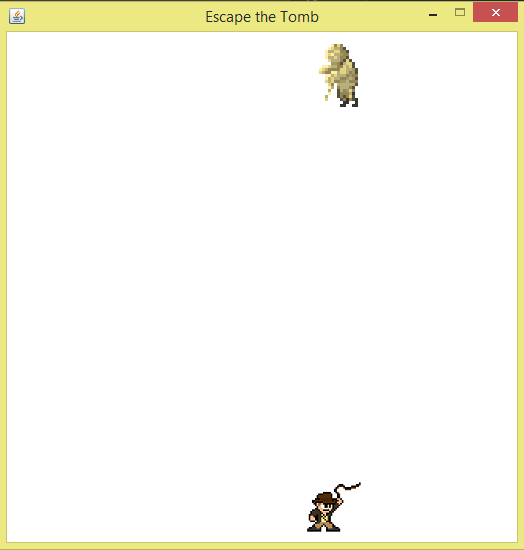
\includegraphics[scale=0.7]{image/field1.png}
		\caption{Игровое поле с расположенными на нём игровыми персонажами} 
		\label{pic:pic_name} % название для ссылок внутри кода
	\end{center}
\end{figure}

Игра заканчивается в двух случаях: либо при достижении археологом выхода, либо при его столкновении с мумией.\\

Мумия заблокирована преградой, поэтому игрок может сделать к мумии несколько шагов, не боясь проиграть, как на рисунке 3:

\begin{figure}[H]
	\begin{center}
		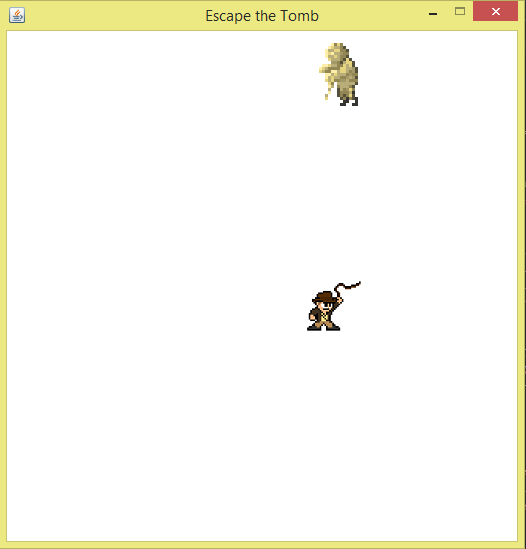
\includegraphics[scale=0.7]{image/field2.png}
		\caption{Мумия не может пройти к игроку} 
		\label{pic:pic_name} % название для ссылок внутри кода
	\end{center}
\end{figure}

Победа будет засчитана, когда персонаж доберётся до выхода, как на рисунке 4. В данном случае выход находится в левом нижнем углу поля. 

\begin{figure}[H]
	\begin{center}
		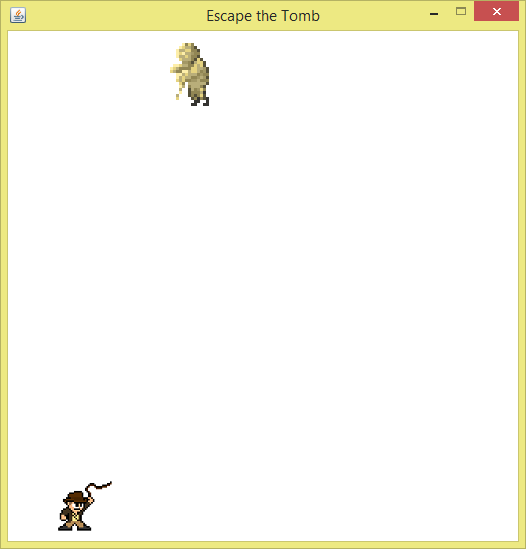
\includegraphics[scale=0.7]{image/field3.png}
		\caption{Игрок добрался до выхода} 
		\label{pic:pic_name} % название для ссылок внутри кода
	\end{center}
\end{figure}

Также игрок может быть пойман мумией, в результате чего он проиграет, как на рисунке 5.

\begin{figure}[H]
	\begin{center}
		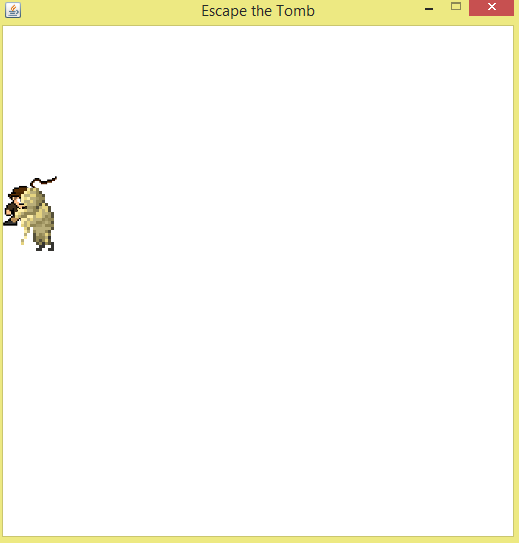
\includegraphics[scale=0.7]{image/field4.png}
		\caption{Декорирование главного экрана} 
		\label{pic:pic_name} % название для ссылок внутри кода
	\end{center}
\end{figure}

При обоих исходах будет выведена на экран надпись Game over. Рисунок 6:

\begin{figure}[H]
	\begin{center}
		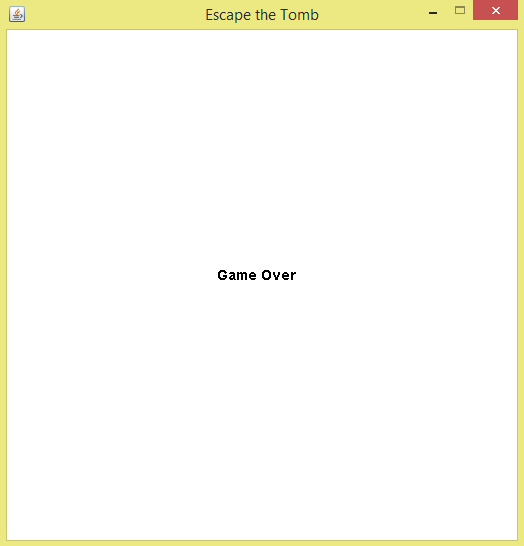
\includegraphics[scale=0.7]{image/gameover.png}
		\caption{Игра окончена} 
		\label{pic:pic_name} % название для ссылок внутри кода
	\end{center}
\end{figure}

Таким образом разработано графическое приложение, позволяющее играть в "Побег из гробницы".\\

\subsection{Вывод}

Для реализации игры определены основные классы библиотеки, графи-
ческого приложения. Разработано графическое приложение, предоставля-
ющее возможность играть одному игроку.\\



\section{Вывод}

В результате работы было разработано игровое приложение "Побег из гробницы". Посредством библиотеки Swing было создано приложение, предоставляющее пользователю функциональность
ядра и позволяющее играть в игру ”Побег из гробницы”.



\section{Приложение}



\subsection{Листинги}


\lstinputlisting{../src/logic/Cell.java}

\lstinputlisting{../src/logic/Field.java}

\lstinputlisting{../src/logic/Player.java}

\lstinputlisting{../src/GUI/Sprite.java}

\lstinputlisting{../src/GUI/Game.java}

\lstinputlisting{../src/GUI/KeyInputHandler.java}

\end{document}
